\documentclass[12pt, a4paper]{article}
\usepackage{fontspec}
\setmainfont{Times New Roman}
\usepackage[UTF8]{ctex}
\usepackage{listings}
\usepackage{array}
\usepackage{geometry}
\geometry{a4paper, scale=0.75}
\usepackage{ctex}
\usepackage{amsmath}
\usepackage{epsfig}
\usepackage{graphicx}
\usepackage{epstopdf}
\usepackage{cite}
\usepackage{indentfirst}
\setlength{\parindent}{2em}
\setlength\parskip{.3 \baselineskip}
\usepackage{graphicx}
\usepackage{float}
\usepackage{subfigure}

\begin{document}
	\begin{center}
		\vspace{0.2in}
		\noindent{\fontsize{20pt}{1em}\selectfont\textbf{通信电路\quad 第七周作业}} \\ [12pt]
		\noindent{\fontsize{20pt}{1em}\textbf{Cadence报告}}  \\ [12pt]
		{\fontsize{14pt}{1.2em}\selectfont
			刘开济\\ [10pt]
			2019010973 \\ [10pt]
		}
	\end{center}
    \section{正交调制/解调电路研究}
    正交调制/解调原理图如下:
        \begin{figure}[H]
    	\centering
    	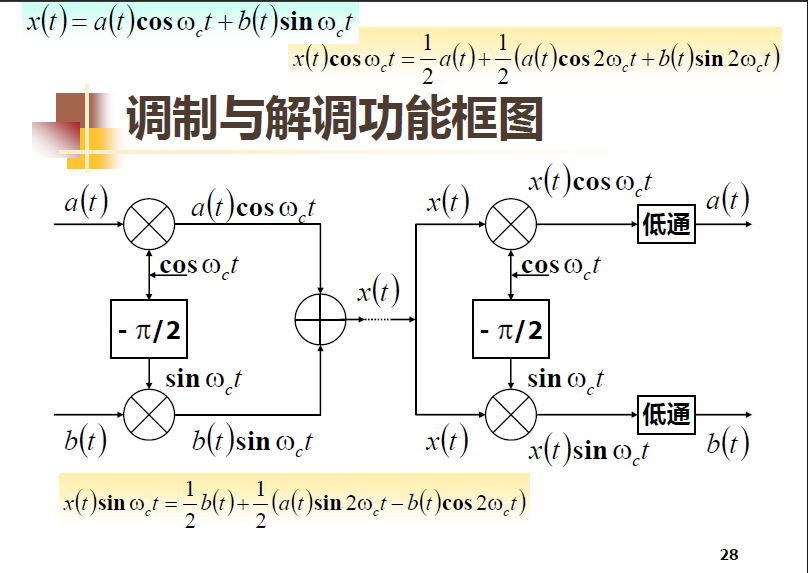
\includegraphics[width = 0.8\textwidth]{theory}
    	\caption{正交调制/解调原理框图}
    \end{figure}\par
    首先设计能够产生I/Q两路脉冲的数字电路,注意到:
    \begin{gather}
    	01001100 = 11001100 \ AND \ 01111111\\
    	10100110 = (11111100 \ XNOR\  10101010)\  XNOR \ 11110000 
    \end{gather}\par
    于是可以设计相应数字信号发生器。
    $90^{\circ}$移相器采用双RC电路构造,比较简单。电路设计如下:
     \begin{figure}[H]
    	\centering
    	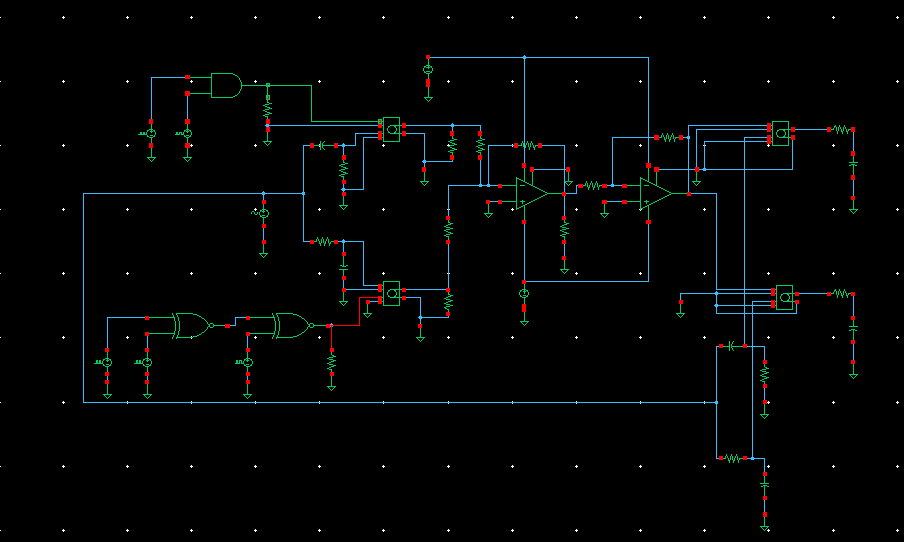
\includegraphics[width = 0.8\textwidth]{circ}
    	\caption{原型电路设计}
    \end{figure}\par
    考察IQ两路输入信号与解调信号,仿真如下:
        \begin{figure}[H]
    	\centering
    	\subfigure[原始信号01001100脉冲]{
    		\begin{minipage}[t]{0.48\linewidth}
    			\centering
    			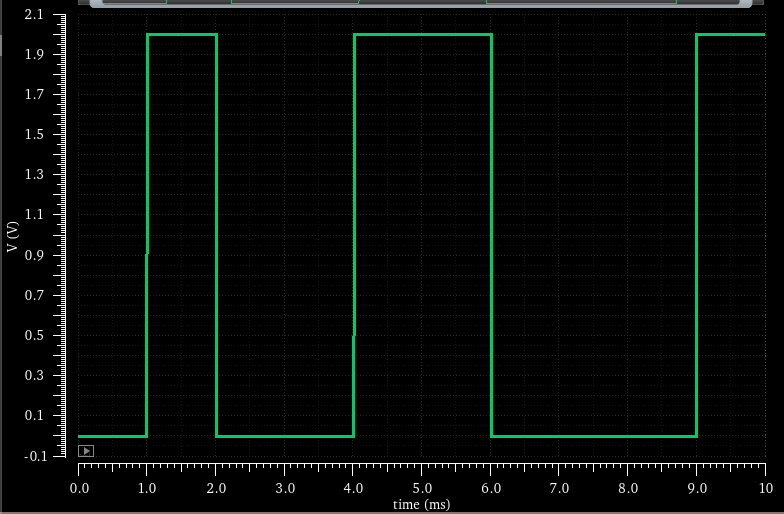
\includegraphics[width=6cm]{01001100}
    		\end{minipage}%
    	}%
    	\subfigure[原始信号10100110脉冲]{
    		\begin{minipage}[t]{0.48\linewidth}
    			\centering
    			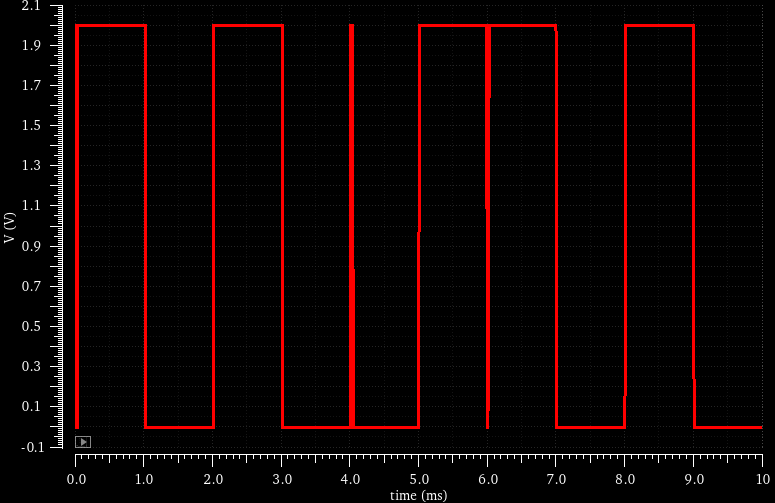
\includegraphics[width=6cm]{10100110}
    		\end{minipage}%
    	}%
    	%这个回车键很重要 \quad也可以 
    	\par
    	\subfigure[解调后01001100波形]{
    		\begin{minipage}[t]{0.48\linewidth}
    			\centering
    			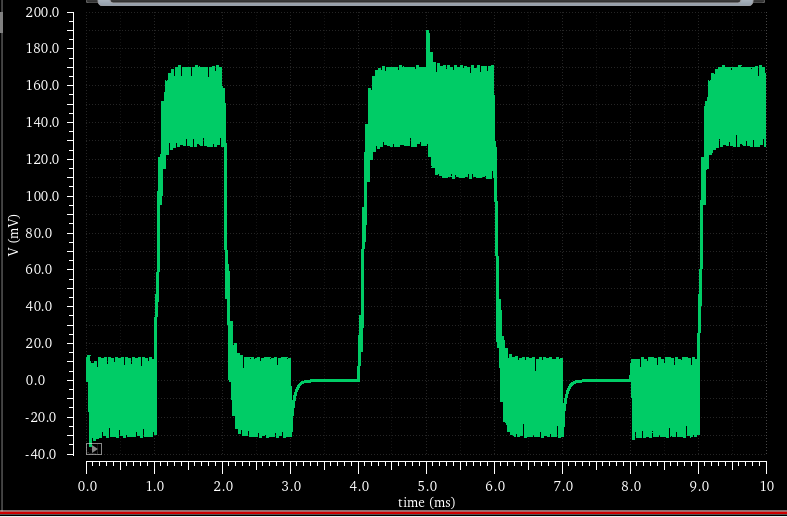
\includegraphics[width=6cm]{rec-01001100}
    		\end{minipage}
    	}%
    	\subfigure[解调后10100110波形]{
    		\begin{minipage}[t]{0.48\linewidth}
    			\centering
    			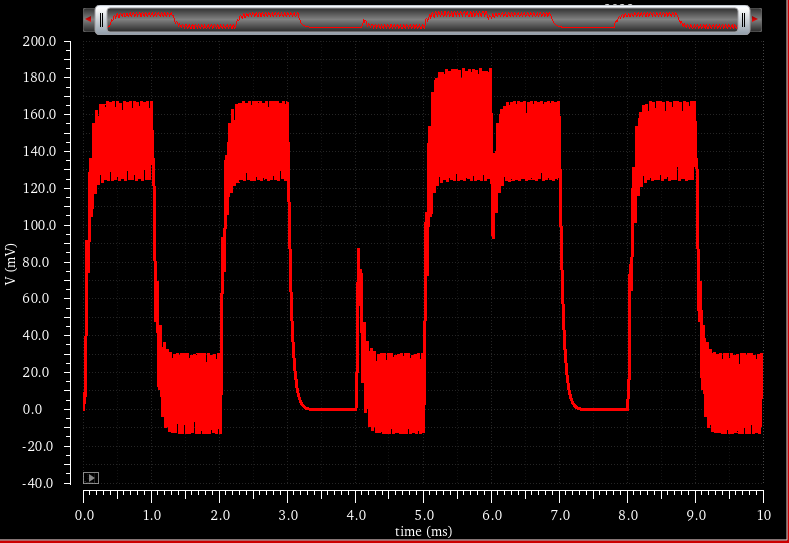
\includegraphics[width=6cm]{rec-10100110}
    		\end{minipage}
    	}%
    	
    	\centering
    	\caption{四种基本放大器交流增益分析}
    \end{figure}\par
\end{document}